2. \begin{figure}[ht!]
\center{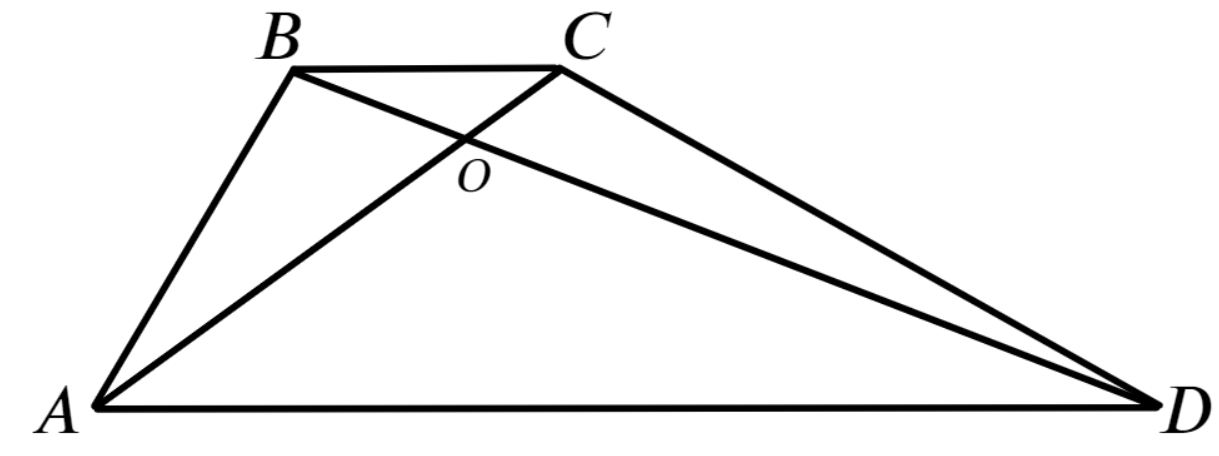
\includegraphics[scale=0.35]{g8-105.png}}
\end{figure}\\
Треугольники $BOC$ и $AOD$ подобны по двум углам ($\angle AOD$ и $\angle BOC$ вертикальные, $\angle BCO$ и $\angle OAD$ накрест лежащие). Раз
$\cfrac{S_{\Delta BOC}}{S_{\Delta AOD}}=\cfrac{1}{81},$ коэффициент подобия равен $\sqrt{\cfrac{1}{81}}=\cfrac{1}{9},$ поэтому $\cfrac{AD}{BC}=9.$\\
